\section{Auswertung}

Fehler und Ausgleichsrechnungen werden mit den Python-Paketen SciPy \cite{scipy} und uncertainties \cite{uncertain} berechnet.

\subsection{Amplitudenmodulation mit Ringmodulator}

Mit dem Ringmodulator wird die Amplitude eines Signals moduliert. Das Eingans- und Ausgangssignal sind in \autoref{a} zu sehen. Das Trägersignal hatte eine Amplitude von $U_\text{T}=\SI{980}{\milli\volt}$ und die Frequenz $\omega_\text{T}=\SI{1}{\mega\hertz}$, das Modulationssignal hatte eine Amplitude von $U_\text{M}=\SI{116}{\milli\volt}$ und die Frequenz $\omega_\text{M}=\SI{50}{\kilo\hertz}$. Es entsteht eine Schwebung, es wird also keine Leistung zur Übertragung des Trägersignals verbraucht; die Trägerfrequenz ist ist als hochfrequenter Anteil im gelben Signal zu erkennen. \par
\indent Die prominentesten Linien in dem Frequenzspektrum in \autoref{b} sind die der Modulationsfrequenz $f_\text{T} \pm f_\text{M}$. Sie liegen bei $f_\text{T} - f_\text{M} = \SI{951.9}{\kilo\hertz}$ und $f_\text{T} + f_\text{M} = \SI{1.0521}{\mega\hertz}$. Erwartet werden $f_\text{T} - f_\text{M} = \SI{950}{\kilo\hertz}$ und $f_\text{T} + f_\text{M} = \SI{1.05}{\mega\hertz}$. Dazwischen ist als kleinerer Peak auch die Trägerfrequenz $f_\text{T} = \SI{1.002}{\mega\hertz}$ zu sehen, die mit dem Ringmodulator nicht komplett unterdrückt wird, aber signifikant kleiner als die Seitenbänder ist. Die Werte werden mit größerer Genauigkeit gemessen, als sie eingestellt werden konnten und stimmen gut mit den jeweils eingestellten Frequenzen überein. \par

\begin{figure}
	\centering
	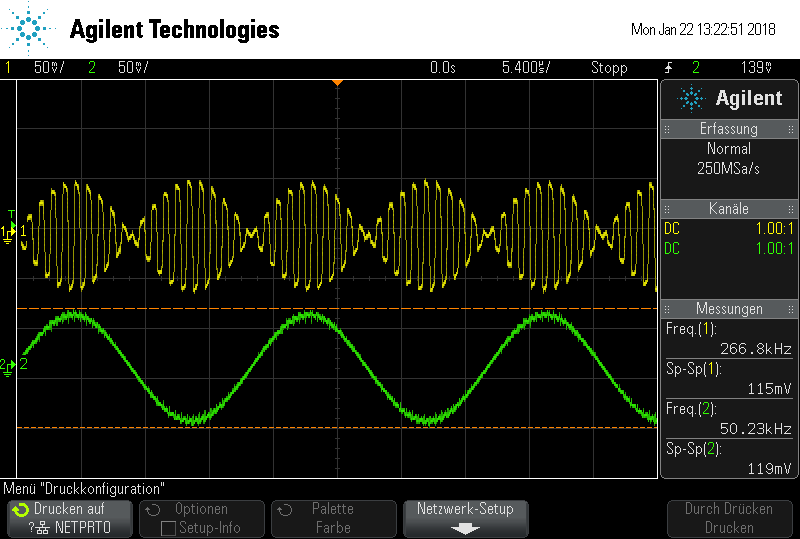
\includegraphics[width=\textwidth]{img/a_scope_230.png}
	\caption{Amplitudenmodulation ohne Trägerabstrahlung - grün das Eingangssignal, gelb das amplitudenmodulierte Signal}
	\label{a}
\end{figure}

\begin{figure}
	\centering
	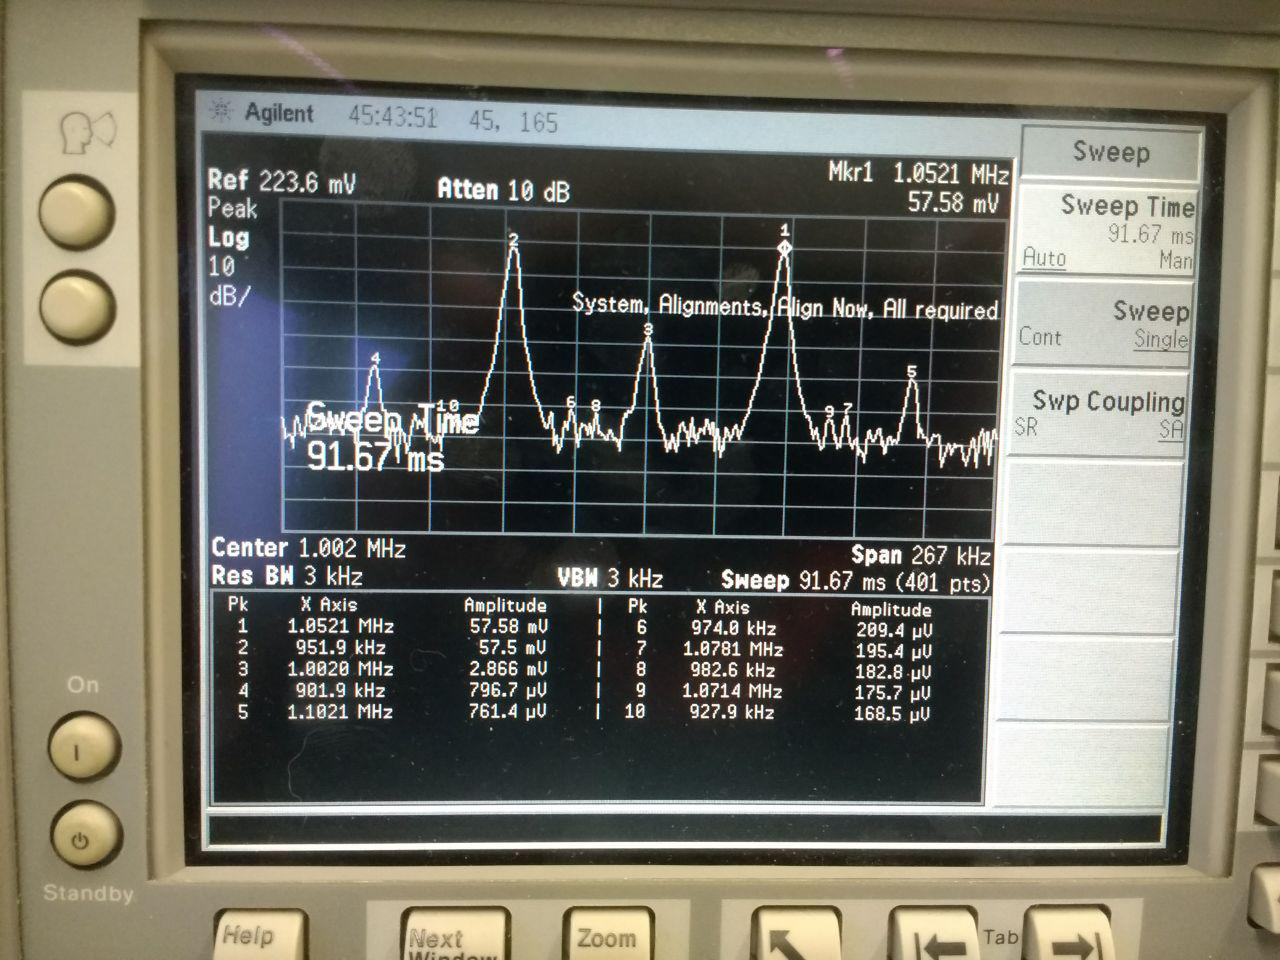
\includegraphics[width=\textwidth]{img/Aufgabenteil_b.jpg}
	\caption{Amplitudenmodulation ohne Trägerabstrahlung - Peak 3 mit der Trägerfrequenz, Peak 1 und 2 die Seitenbänder}
	\label{b}
\end{figure}

\subsection{Amplitudenmodulation mit Tr\"{a}gerabstrahlung}

In \autoref{c1} ist das Fequenzspektrum einer amplitudenmodulierten Schwingung mit Trägerabstrahlung zu sehen. Das Trägersignal hatte eine Amplitude von $U_\text{T}=\SI{1.17}{\volt}$ und die Frequenz $\omega_\text{T}=\SI{1.55}{\mega\hertz}$, das Modulationssignal hatte eine Amplitude von $U_\text{M}=\SI{159}{\milli\volt}$ und die Frequenz $\omega_\text{M}=\SI{63}{\kilo\hertz}$. \autoref{c2} zeigt von dem gleichen Signal eine Oszilloskop-Aufnahme. In \autoref{c2} lässt sich der Modulationsgrad aus dem Verhältnis der Amplitude der Maxima und der Minima bestimmen. Da die Amplitude zwischen $U_\text{min} = U_\text{T}(1 - m)$ und $U_\text{max} = U_\text{T}(1 + m)$ schwankt, ist der Modulationsgrad nach
\[
	m = \frac{U_\text{max} - U_\text{min}}{U_\text{max} + U_\text{min}}
\]
mit $U_\text{min} = \SI{24}{\milli\volt}$ und $U_\text{max} = \SI{54}{\milli\volt}$, wobei die Spannungswerte mit einer Unsicherheit von $\pm \SI{2}{\milli\volt}$ angegeben werden, $m = 0.38 \pm 0.04$.\par
\indent Der Modulationsgrad kann auch mit der Pulshöhe der Träger- und Modulationsfrequenz bestimmt werden, welche an dem Frequenzanalysator abgelesen werden kann. Dazu wird die Pulshöhe, die in der Einheit eines Leistungspegels $L_P$ angegeben wird, mit $P = 10^{L_P/10} \cdot \SI{1}{\milli\watt}$ in eine Leistung umgerechet. $L_P$ wird mit einer Genauigkeit von $\SI{0.01}{\dBm}$ gemessen. Die Leistung hängt mit der Spannung über $P = U^2/2R$ zusammen. Die Leistung des Trägersignals $P_\text{T}$ und der Seitenbänder $P_\text{S}$ ist
\[
P_\text{T} = \frac{U_\text{T}^2}{2R} \quad \text{und} \quad P_\text{S} = \frac{\left(\frac{m \cdot U_\text{T}}{2}\right)^2}{2R} = \frac{m^2 \cdot {U_\text{T}^2}}{8R}.
\]
Dann ist der Modulationsgrad
\[
	m = \sqrt{4 \cdot \frac{P_\text{M}}{P_\text{T}}} = \sqrt{4 \cdot \frac{10^{L_{P,\text{M}}/10}}{10^{L_{P,\text{T}}/10}}}
\]
mit $P_\text{M,1} = \SI{-44.62}{\dBm}$, $P_\text{M,2} = \SI{-44.70}{\dBm}$ und $P_\text{T} = \SI{-33.68}{\dBm}$ $m_1 = 0.5676 \pm 0.0009$ bzw. $m_2 = 0.5624 \pm 0.0009$.
Der Unterschied zwischen dem berechneten Modulationsgrad mit beiden Methoden beträgt 68\%.

\begin{figure}
	\centering
	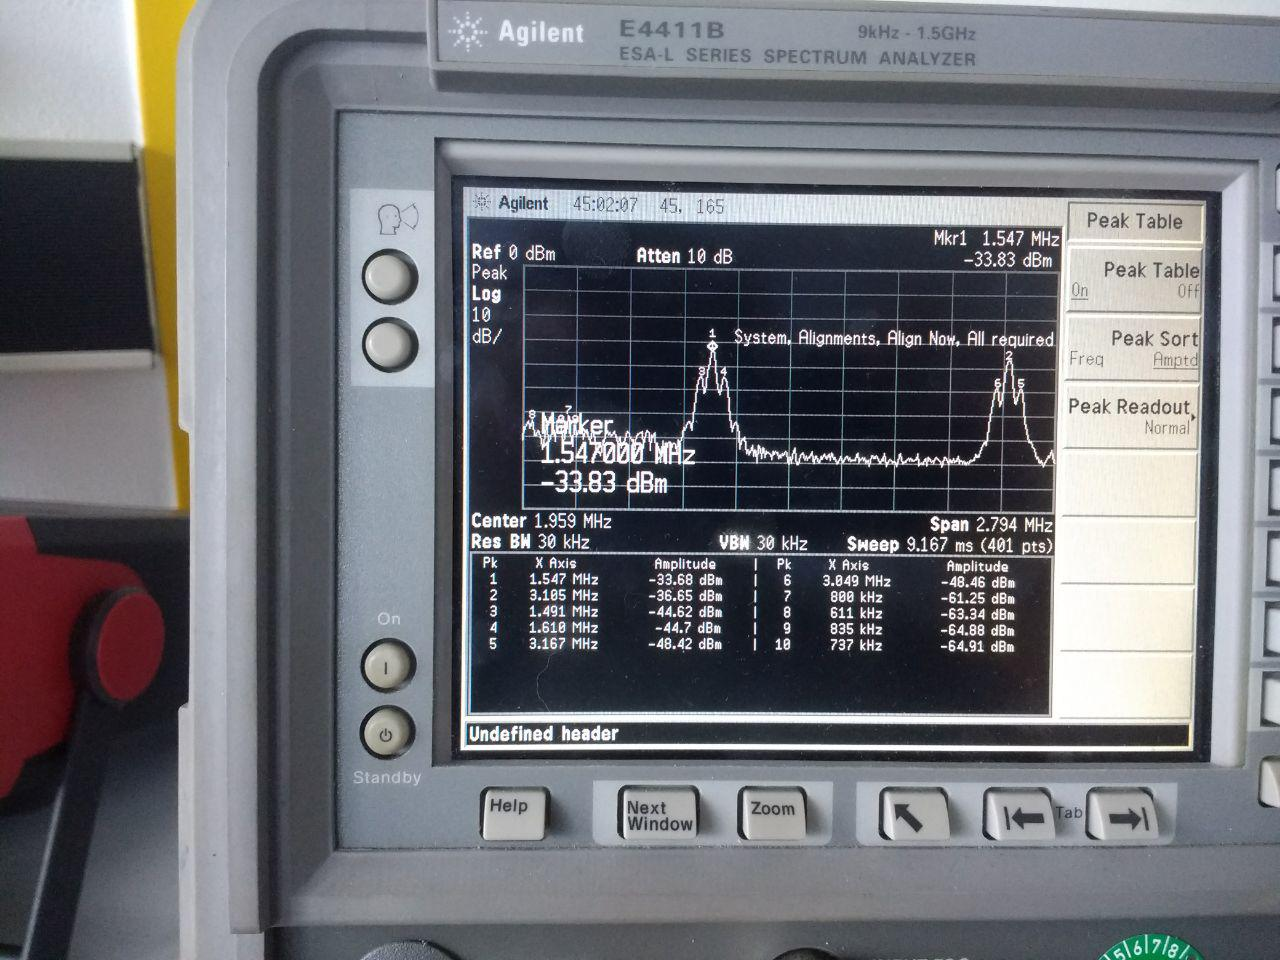
\includegraphics[width=\textwidth]{img/Aufgabenteil_c1.jpg}
	\caption{Amplitudenmodulation mit Trägerabstrahlung -- es sind Oberwellen und Seitenbänder zu sehen.}
	\label{c1}
\end{figure}

\begin{figure}
	\centering
	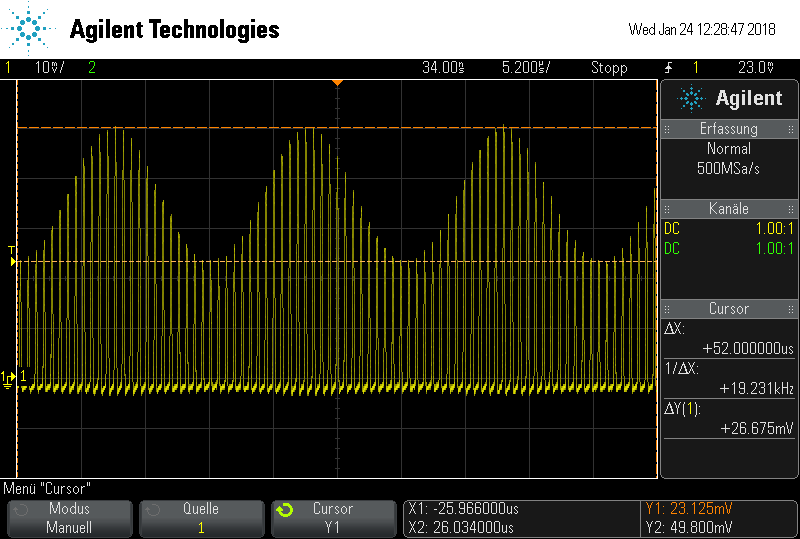
\includegraphics[width=\textwidth]{img/c_scope_247.png}
	\caption{Amplitudenmodulation mit Trägerabstrahlung -- Bestimmung des Modulationsgrades}
	\label{c2}
\end{figure}

\subsection{Frequenzmodulation}

Das Trägersignal hatte eine Amplitude von $U_\text{T}=\SI{320}{\milli\volt}$ und die Frequenz $\omega_\text{T}=\SI{875}{\kilo\hertz}$, das Modulationssignal hatte eine Amplitude von $U_\text{M}=\SI{320}{\milli\volt}$ und die Frequenz $\omega_\text{M}=\SI{180}{\kilo\hertz}$. Die Breite der Verschmierung in \autoref{d1} ist an der maximalen Stelle $\Delta t = \SI{196}{\nano\second}$. Dies verteilt sich auf fünf Perioden, also $\Delta \bar{t} = \SI{39.2}{\nano\second}$.
Die Integration der Momentanfrequenz aus \autoref{eq:momFreq} in den Grenzen von $0$ bis $T_\text{M}/2$ geteilt durch die Länge des Integrationsintervalls ergibt für die Phase $\varphi = \pi$ bzw. $\varphi = 0$ jeweils die extremalen, über eine halbe Periode gemittelte Momentanfrequenz
\[
	\bar{f}_\text{mom} = \frac{2}{T_\text{M}} \cdot f_\text{T}\int_0^{T_\text{M}/2} 1 - m \cdot \sin (\omega_\text{M} t + \varphi) \,dt = f_\text{T}\left( 1 \pm \frac{2m}{\pi} \right).
\]
Aus der Differenz des Kehrwerts der beiden gemittelten Momentanfrequenzen ergibt sich die mittlere Verschmierung $\Delta \bar{t}$
\[
	\frac{1}{f_1} - \frac{1}{f_2} = \Delta \bar{t}.
\]
Dies lässt sich umformen zu
\[
	m(\Delta \bar{t}) = \frac{\pi}{2f_\text{t}\Delta \bar{t}} \left( -1 \pm \sqrt{ 1 + {f_\text{T}}^2 \Delta \bar{t}^2} \right),
\]
wobei nur die positive Lösung als physikalisch sinnvoll betrachtet wird. Daraus ergibt sich der Modulationsgrad $m = 0.134 \pm 0.003$. Für $\Delta \bar{t}$ wurde eine Unsicherheit von $\SI{5}{\nano\second}$ angenommen und für $f_\text{T}$ eine Unsicherheit von $\SI{2}{\kilo\hertz}$.

\begin{figure}[t!]
	\centering
	\begin{subfigure}[t]{0.48\textwidth}
		\centering
		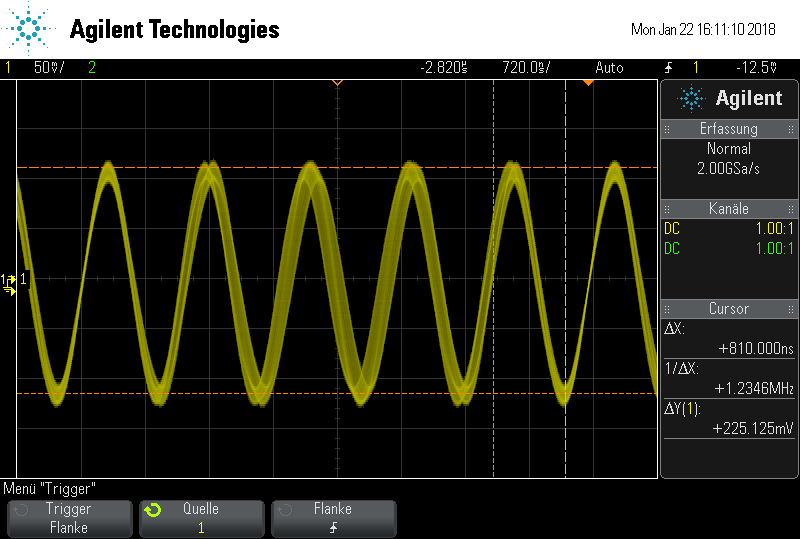
\includegraphics[width=\textwidth]{img/d_scope_233.png}
		\caption{Frequenzmodulation}
	\end{subfigure}\hfill%
	\begin{subfigure}[t]{0.48\textwidth}
		\centering
		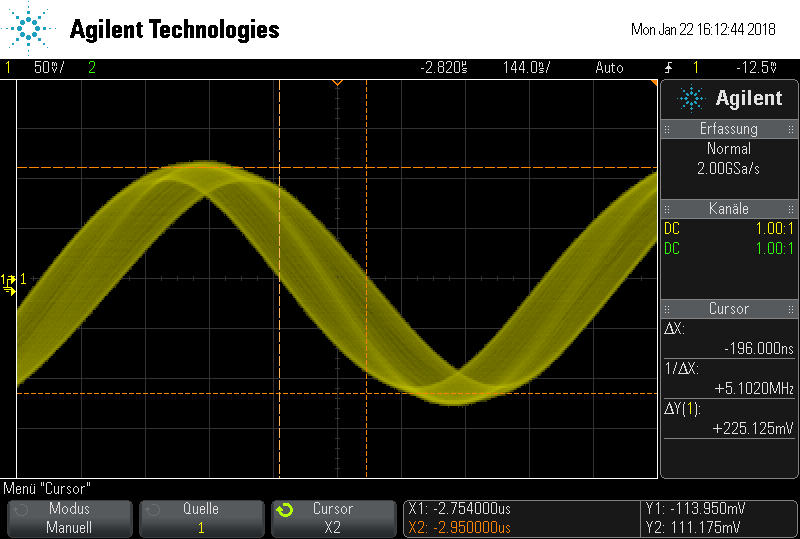
\includegraphics[width=\textwidth]{img/d_scope_234.png}
		\caption{Frequenzmodulation -- Detailansicht zur Bestimmung der Breite der Verschmierung}
	\end{subfigure}
	\caption{Frequenzmodulation eines sinusförmigen Trägersignals.}
	\label{d1}
\end{figure}

\begin{figure}
	\centering
	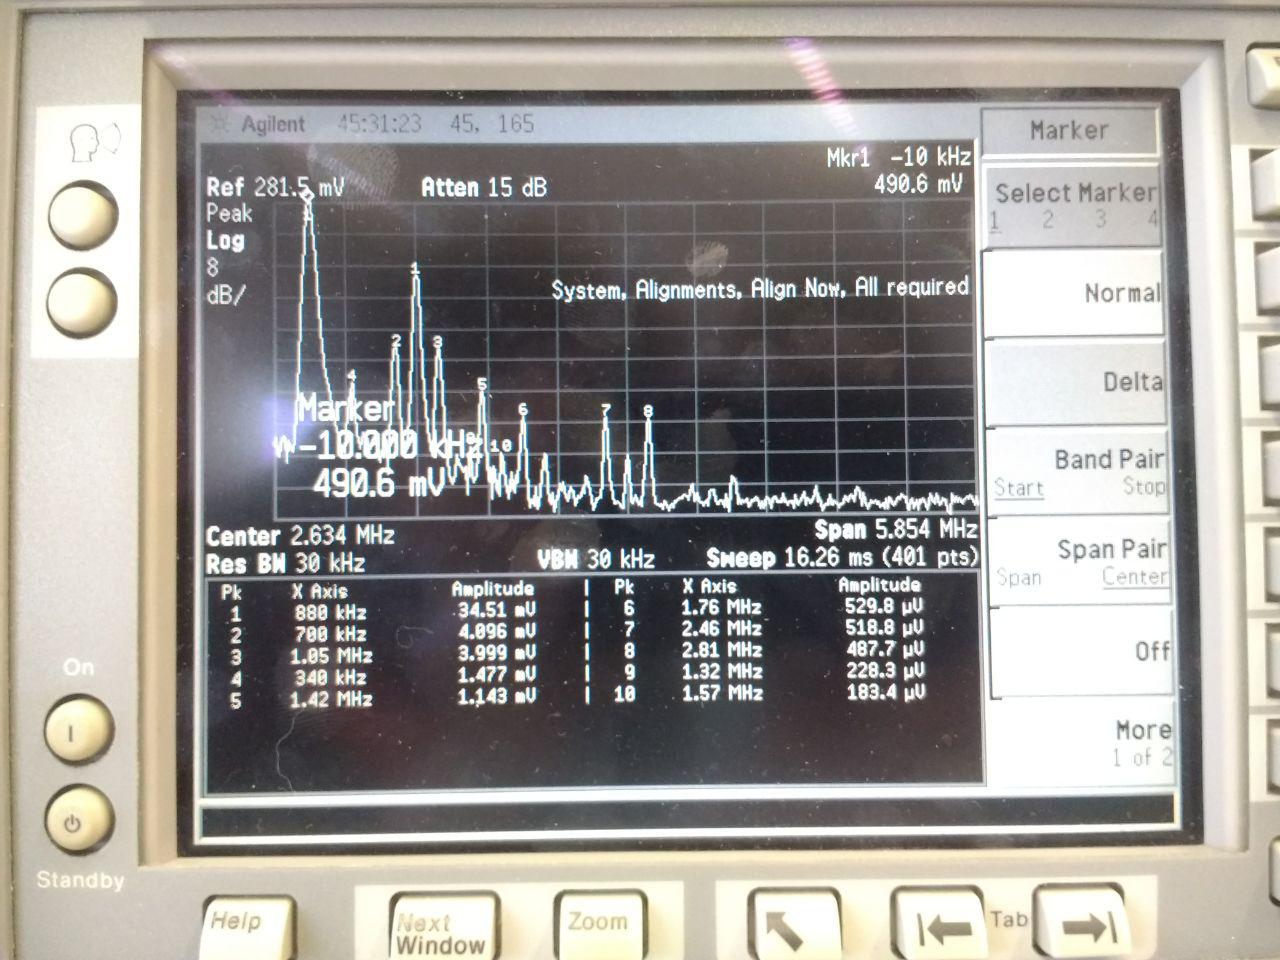
\includegraphics[width=\textwidth]{img/Aufgabenteil_d.jpg}
	\caption{Frequenzmodulation -- Frequenzspektrum}
	\label{d2}
\end{figure}

\subsection{Proportionalit\"{a}t zwischen Gleichspannung am Ausgang und Phase der Wechselspannung zwischen den Eing\"{a}ngen am Ringmodulator}

Die Annahme ist, dass eine Proportionalität zwischen der Gleichspannung $U_\text{A}$ am Ausgang X des Ringmodulators in \autoref{Abb14} und der Phase $\varphi$ der Wechselspannung an den Eingängen R und L des Ringmodulators besteht. Um diesen Zusammenhang zu überprüfen, wird die Gleichspannung in Abhängikeit des Arguments des Cosinus gemessen. Es kann entweder die Laufzeit $\Delta T$ oder die Frequenz des Trägersignals $\omega_\text{T}$ variiert werden. In diesem Fall wird die Frequenz verändert, sodass

\begin{align}
\begin{split}
	U_\text{A} &= \gamma U_0 \cos(\omega_T \cdot \Delta T + \varphi_0)\\
	\arccos \frac{U_\text{A}}{\gamma U_0} &= \omega_T \cdot \Delta T + \varphi_0
\end{split}
\end{align}

gelten muss.

Eine lineare Ausgleichsrechnung der Form $\arccos (\hat{U}) = A \cdot \omega_\text{T} \cdot \Delta T + \varphi_0$ an die Messwerte in \autoref{tab:e} ergibt die Parameter $A = -1.41 \pm 0.07$ und $\varphi_0 = 3.37 \pm 0.09$ und ist in \autoref{fig:e} dargestellt. In $A$ werden Effekte zusammengefasst, die sich auf Frequenz und Laufzeit auswirken und nicht identifizierbar sind, $\varphi_0$ ist ein konstanter Phasenoffset. Die geringen Fehler des linearen Fits von 5.0\% für die Steigung bzw. 2.8\% für den y-Achsenabschnitt zeigen, dass die Annahme eines ein linearen Zusammenhangs gerechtfertig ist.

\begin{figure}
	\centering
	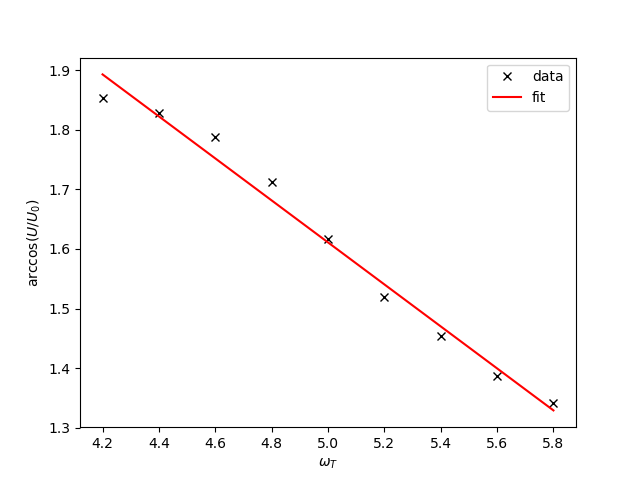
\includegraphics[width=\textwidth]{img/linear_fit.png}
	\caption{Lineare Ausgleichsrechnung zur Veranschaulichung des linearen Zusammenhangs zwischen $\cos\varphi$ und $U$.}
	\label{fig:e}
\end{figure}

\subsection{Demodulation einer amplitudenmodulierten Schwingung mit Ringmodulator}

In \autoref{f} ist die Oszilloskop-Aufnahme eines Signals zu sehen, dessen Amplitude zunächst moduliert und daraufhin wieder demoduliert wird. Das in gelb dargestellte Signal ist das Eingangssignal, die grüne Kurve ist das um einen festen Faktor phasenverschobene und in der Amplitude reduzierte demodulierte Signal. Das Eingangssignal wurde mit einem Ringmodulator gemäß der Schaltung in \autoref{iso-t} demoduliert.

\begin{figure}
	\centering
	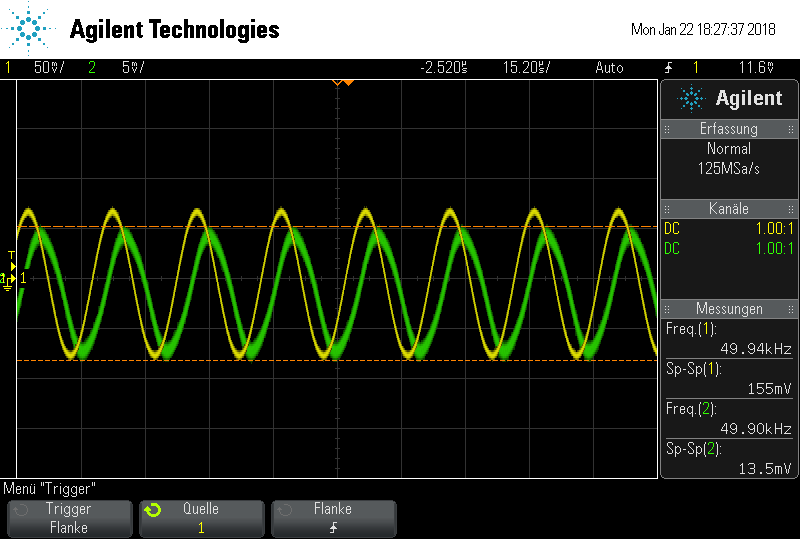
\includegraphics[width=\textwidth]{img/f_scope_235.png}
	\caption{Amplituden(de-)modulation -- gelb das Eingangssignal, grün das amplitudenmodulierte und daraufhin mit einem Ringmodulator demodulierte Signal}
	\label{f}
\end{figure}

\subsection{Demodulation mit Gleichrichterdiode}
\label{De-AM}

Die Diode in der Schaltung in \autoref{fig:9} schneidet die negativen Halbwellen ab, wie in \autoref{nachDiode} zu sehen und das RC-Element filtert als Tiefpass die hohen Frequenzen aus dem Signal, dies ist in \autoref{nachRC} zu sehen. Wie zu erwarten ist die Amplitude des Ausgangsignal nach dem Tiefpass stark reduziert und das Ausgangssignal ist gegenüber dem Eingangssignal phasenverschoben. Es ist außerdem durch die Modulation eine Verdopplung der Frequenz zustande gekommen, da bei dieser eine Schwebung entsteht, von der durch die Diode die untere Einhüllende abgeschnitten wird.

\begin{figure}[t!]
	\centering
	\begin{subfigure}[t]{0.48\textwidth}
		\centering
		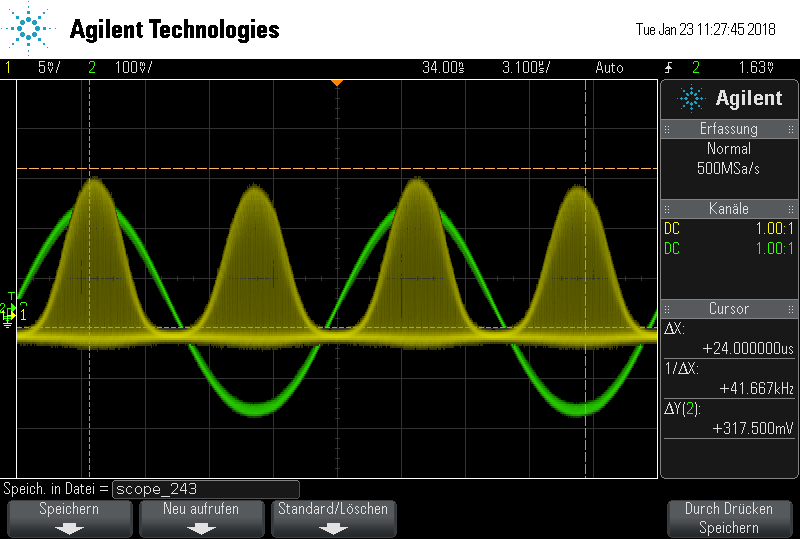
\includegraphics[width=\textwidth]{img/g_scope_243.png}
		\caption{Das Eingangssignal ist in grün abgebildet, in gelb das Signal nach der Diode in der Schaltung in \autoref{fig:9}.}
		\label{nachDiode}
	\end{subfigure}\hfill%
	\begin{subfigure}[t]{0.48\textwidth}
		\centering
		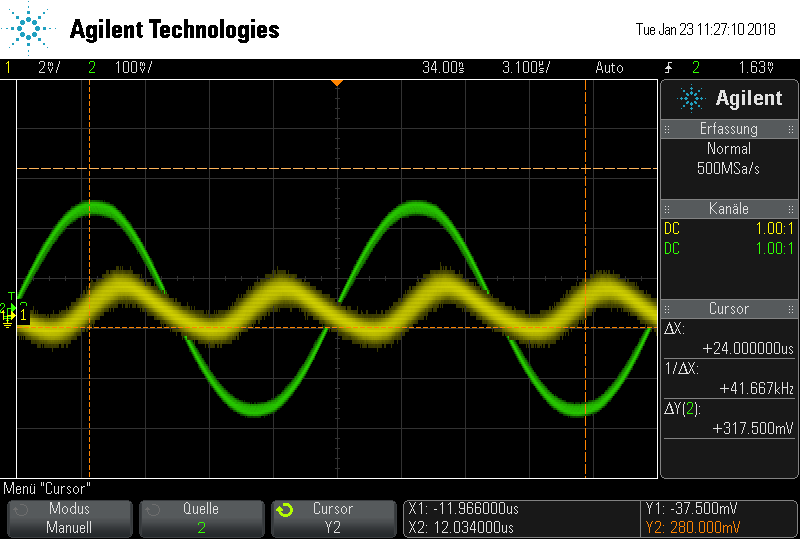
\includegraphics[width=\textwidth]{img/g_scope_242.png}
		\caption{Das Einganssignal ist wieder in grün, in gelb das demodulierte Ausgangssignal nach dem Tiefpass.}
		\label{nachRC}
	\end{subfigure}
	\caption{Demodulation eines amplitudenmodulierten Signals mit einer Gleichrichterdiode.}
\end{figure}

\subsection{Demodulation einer frequenzmodulierten Schwingung}

In \autoref{amp} ist mit der Schaltung in \autoref{gleichrichter} aus dem frequenzmodulierten Signal eine Amplitudenmodulation gemacht worden. \autoref{De-FM} und \autoref{De-FM-RC} zeigen die anschließende Demodulation mit einer Gleichrichterdiode und einem RC-Tiefpass wie bereits in \autoref{De-AM} durchgeführt.
Anhand der Schwebung wird deutlich, dass die Umwandlung von Frequenz- zu Amplitudenmodulation erfolgreich war. Mit der Gleichrichterdiode wrden die negativen Halbwellen abgeschnitten, es sind allerdings noch hochfrequente Störungen im Signal vorhanden. Diese werden mit einem Tiefpass herausgefiltert, was jedoch zu einer starken Abnahme der Amplitude führt.

\begin{figure}[t!]
	\centering
	\begin{subfigure}[t]{0.48\textwidth}
		\centering
		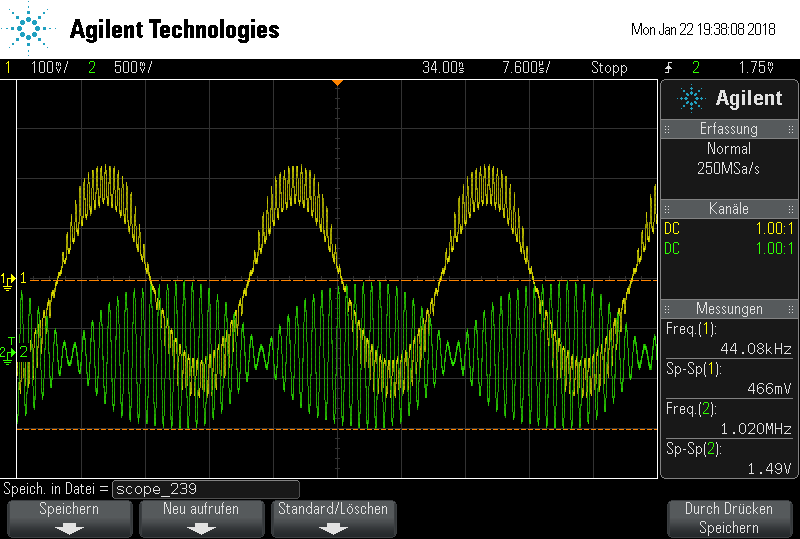
\includegraphics[width=\textwidth]{img/h_scope_239.png}
		\caption{In gelb ist das Eingangssignal gezeigt, in grün das modulierte Signal -- durch den LC-Kreis wird aus der frequenzmodierten Spannung ein amplitudenmoduliertes Signal.}
		\label{amp}
	\end{subfigure}\hfill%
	\begin{subfigure}[t]{0.48\textwidth}
		\centering
		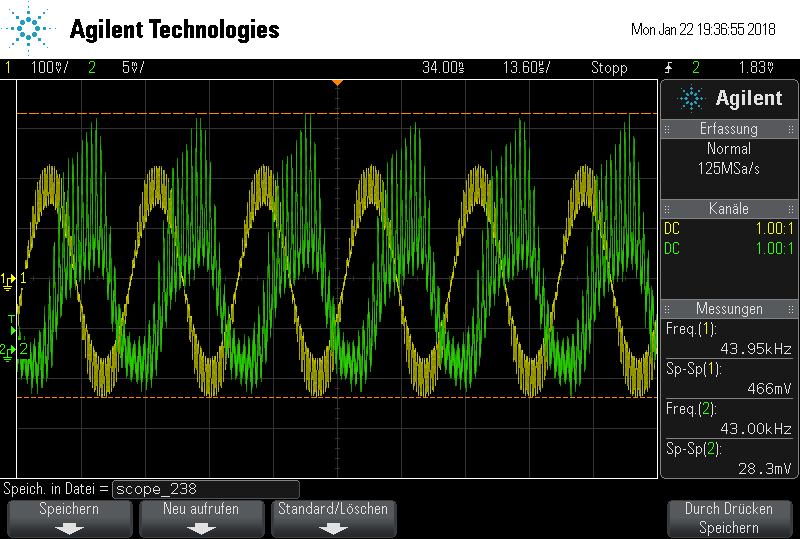
\includegraphics[width=\textwidth]{img/h_scope_238.png}
		\caption{Mit einer Gleichrichterdiode werden die negativen Halbwellen abgeschnitten.}
		\label{De-FM}
	\end{subfigure}
	\\
	\begin{subfigure}[t]{0.5\textwidth}
		\centering
		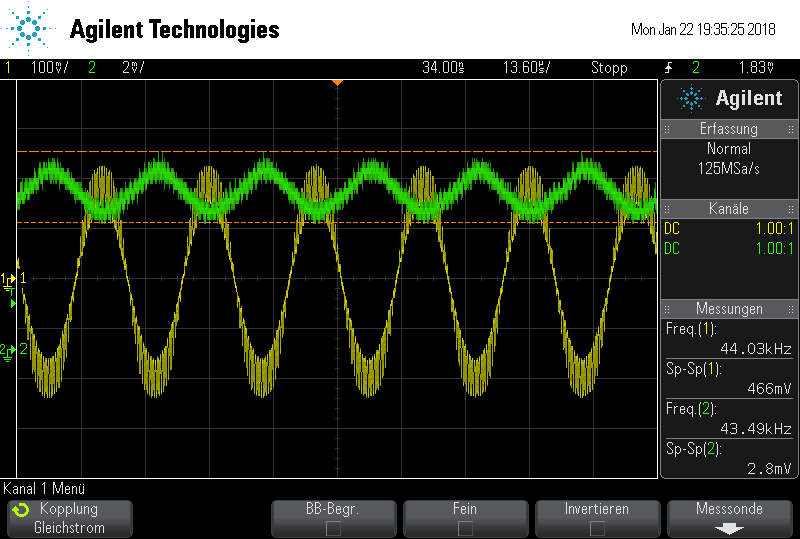
\includegraphics[width=\textwidth]{img/h_scope_237.png}
		\caption{Das in grün dargestellte Signal ist demoduliert und wurde nach dem Tiefpass abgegriffen.}
		\label{De-FM-RC}
	\end{subfigure}
	\caption{Demodulation einer frequenzmodulierten Schwingung.}
\end{figure}

\FloatBarrier
